\documentclass[spanish, 12pt, letterpaper]{article}
\usepackage[utf8]{inputenc}
\usepackage[letterpaper,left=3.0cm,right=3.0cm,top=2.5cm,bottom=2.5cm]{geometry}
\usepackage{graphicx}
\usepackage[spanish]{babel}
\usepackage[natbibapa]{apacite}
\usepackage{setspace} \onehalfspacing
\usepackage{fontspec}
\usepackage{listings}
\setmainfont{Arial}

\title {
{\Large \textbf{UNIVERSIDAD NACIONAL AUTÓNOMA DE MÉXICO}}\\
{\large ESCUELA NACIONAL PREPARATORIA}\\
\vspace{2cm}
{\Large Desarrollo y evaluación de un robot para el cuidado de plantas mediante sensores y redes neuronales recurrentes: Agrocare}\\
\vspace{1cm}
{\large \textbf{Viña Almeida, Ulises}}\\
{\large \textbf{R.G.K.E.}}\\
\vspace{1cm}
{\normalsize TRABAJO DE INVESTIGACIÓN PARA LA SEXTA COMPETENCIA DE ROBÓTICA DE LA ESCUELA NACIONAL PREPARATORIA}\\
\vspace{2cm}
{\normalsize PROFESORA GUÍA: Milagros Pacheco Castañeda}\\
{\normalsize PROFESOR CO-REFERENTE: Alejandro Nava Álvarez}\\
\vspace{2cm}
{\normalsize FEBRERO 2023}
}

\author{}
\date{}

\renewcommand{\refname}{Bibliografía}
\renewcommand{\contentsname}{Tabla de Contenidos}

\begin{document}

\maketitle
\setcounter{secnumdepth}{0}
\thispagestyle{empty}

\tableofcontents

\newpage

\section{Definición del Problema}

\subsection{Huertos urbanos}

Los huertos urbanos son jardines o cultivos a pequeña escala que buscan producir plantas, frutas y verduras en hogares \citep{gobmx_huertos_urbanos}. Sin embargo, el estilo de vida acelerado y ocupado de las personas suele impedir el cuidado adecuado de las plantas, lo que reduce la producción y puede incluso llevar a la muerte de las plantas. A pesar de esto, los huertos urbanos han ganado popularidad en los últimos años debido a los efectos económicos de la pandemia por Covid-19 y la conciencia ambiental. En Guadalajara, se han creado organizaciones civiles para fomentar la creación y mantenimiento de huertos barriales en la ciudad \citep{huertos_urbanos_gdl}. Sin embargo, esta tendencia no sólo se ha visto en crecimiento en Guadalajara, también en el resto del país, es así que la Ciudad de México se posiciona como la segunda con mayor cantidad de huertos urbanos en latinoamérica \citep{huertos_urbanos_cdmx}.

\subsection{Huertos rurales}

A medida que los huertos rurales crecen en tamaño, surgen desafíos en el cuidado y mantenimiento de los cultivos. Uno de los principales desafíos es la falta de atención constante, lo que es esencial para el cuidado de los cultivos, pero a menudo resulta complicado y costoso. Existen dispositivos tecnológicos para el cuidado y monitoreo de los huertos, pero su alto costo los hace inaccesibles para muchos productores nuevos en la industria. Estos desafíos afectan tanto a los productores como a los consumidores, ya que los precios elevados de los alimentos pueden dificultar el acceso a productos saludables y nutritivos, lo que a su vez afecta la calidad de vida de la población.

Es fundamental encontrar soluciones asequibles y eficaces para los productores urbanos y rurales que permitan mantener la productividad de los huertos sin elevar los precios de los alimentos.

\section{Objetivo del Proyecto}

El objetivo de la presente es determinar si el cuidado de plantas automatizado con robótica es: eficiente, escalable y sostenible a largo plazo. De este modo, se espera que Agrocare pueda ser utilizado para medir los valores que afectan el crecimiento de una planta, que incluyen humedad del suelo, humedad relativa, luz solar y temperatura, posteriormente, estos datos serán analizados en un servidor remoto apoyándose de un microservicio de Red Neuronal Recurrente y una base de datos. Se espera que el flujo de datos sea el siguiente:

\renewcommand{\figurename}{Figura}
\begin{figure}[h]
  \centering
  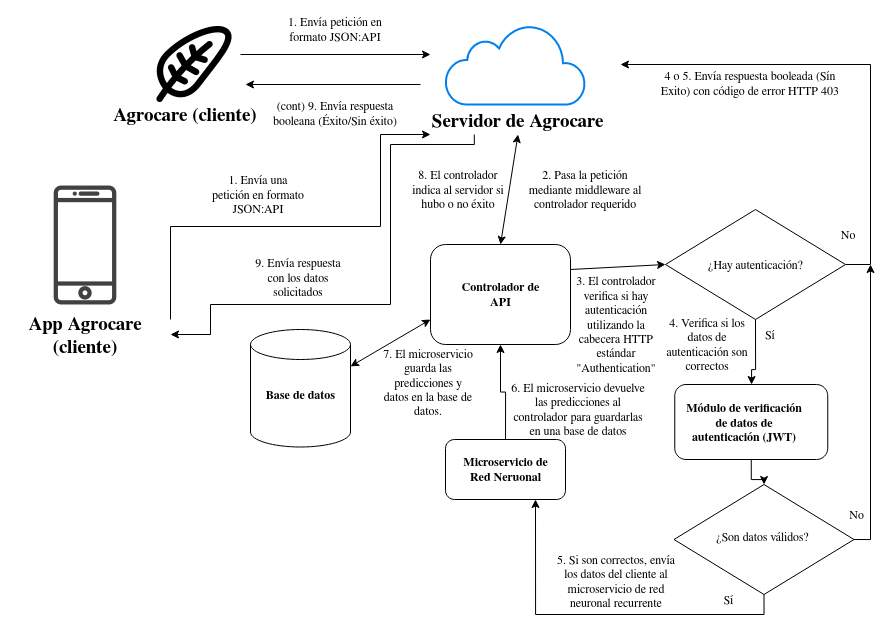
\includegraphics[width=\linewidth]{diagrama.png}
  \caption{Diagrama del flujo de datos}
  \label{fig:example}
\end{figure}

Una vez obtenidos estos datos, se podrá demostrar con datos estadísticos la efectividad de la robótica en la agricultura, que da pie a la posterior utilización de estos sistemas en producción.

\section{Marco Teórico}

Se ha comprobado que la tecnología es muy útil para el cuidado y seguimiento de las plantas. Actualmente, existen diversas tecnologías como los sensores de temperatura y humedad que permiten monitorear y controlar el entorno de las plantas.
\vspace{0.5cm}

Estos sensores pueden conectarse a dispositivos de Internet de las Cosas (IoT), lo que facilita la recolección y análisis de datos en tiempo real, permitiendo tomar decisiones y establecer estrategias para el cuidado de las plantas.
\vspace{0.5cm}

Existen aplicaciones móviles y plataformas en línea que permiten monitoreo y control remoto de los huertos, aprovechando la implementación del IoT. La información recolectada puede ser guardada y procesada por una Red Neuronal Recurrente (RNN) para una proyección de datos basada en datos históricos. La implementación de tecnología en los huertos puede mejorar la productividad y calidad de los cultivos, además de tener un impacto positivo en el medio ambiente. Para este propósito, se determinó que IoT y RNN son útiles ya que el primero envía datos en tiempo real y los usuarios pueden interactuar con ellos, mientras que el segundo ajusta los sesgos utilizando data histórica. Además, el uso de RNN asegura la fidelidad de los datos ya que es utilizada para datos secuenciales, como es el caso de Agrocare.
\vspace{0.5cm}

Existe un trabajo de investigación acerca de la robótica e inteligencia artificial para producción "\textit{Robotics for plant proudction}" \citep{robotics_for_plant_production}, sin embargo este se enfoca en producción masiva por lo que no es viable enfocarlo a huertos urbanos, a pesar de esto, la investigación aporta datos que ayudan a entender cómo es que un sistema de este estilo se comportaría en diferentes ambientes dados sus factores ambientales (algunos no controlables, según el estudio), y culturales, dando pie a la pregunta de si es o no viable utilizar estos sistemas en producción.

\section{Descripción y Funcionamiento del Prototipo}
\subsection{Descripción}
El prototipo de Agrocare está construido con materiales reciclados y equipado con un sistema de cómputo y sensores para monitorear el estado del invernadero. Es un recipiente rectangular de 26x17.4cm (452.4 cm²) que tiene una sección para la planta (~75\% del recipiente) y otra para el agua de riego (~25\% del recipiente).\\

Se utilizan tres tipos de sensores para el monitoreo: el Sensor DHT-11, el Sensor de humedad de suelo capacitivo y la Fotorresistencia. El Sensor DHT-11 mide la temperatura y la humedad del aire, el Sensor de humedad de suelo capacitivo mide la humedad del suelo y la Fotorresistencia mide la intensidad de la luz solar.\\

Se eligió la placa de desarrollo basada en el microcontrolador ESP32, en específico la T-Display de TTGO, debido a su potencia y conectividad Wi-Fi y Bluetooth. Además, esta placa incluye una pantalla LCD de 1.14 pulgadas para mostrar información en tiempo real al usuario final. Se utilizó una batería reciclada de un teléfono Motorola con una capacidad de 2,810 mAh a 3.7V (10.36Wh), alimentada por una celda fotovoltáica de 700 mAh a 17V (11.9Wh), esta última ayuda a que el proyecto sea autosustentable energéticamente.

\subsection{Código}
Para la implementación de la API y el Socket:
\lstset{language=JavaScript}
\begin{lstlisting}[language=JavaScript]
// Previo a esta linea deben importarse las dependencias.
require("dotenv").config();
app.use(cors(),express.json(),express.urlencoded({extended:false}));
app.use("/v1/auth", auth);
app.use("/v1/data", data);
io.attach(server,{pingInterval:10000,pingTimeout:5000,cookie:false});
io.use(socketAuth);
app.listen(port,()=>{console.log(Listening on port ${port})});
\end{lstlisting}
\vspace{0.3cm}
\noindent{El código para los microservicios, microcontrolador, el resto de implementaciones de la API y la app móvil está disponible en la siguiente liga: \href{https://github.com/Agr0care/agrocare}{https://github.com/Agr0care/agrocare}}

\section{Resultados}
Como resultados del prototipo, logramos regar una planta de lentejas utilizando Agrocare, también, como fruto de la investigación recolectamos data de 20 plantas que comúnmente se cultivan en huertos urbanos (Lentejas, Frijoles, Rábanos, Caléndula, Girasoles, Lechuga, Albahaca, Cactus, Orégano, Pimiento, Trigo, Avena, Centeno, Ajo, Guisantes, Lavanda, Tomillo, Margaritas, Claveles, Zanahoria) entre los datos recolectados se encuentra el estrés y déficit hídrico, qué condiciones de luminocidad y temperatura requieren, y qué cuidados especiales requieren.

\renewcommand{\figurename}{Figura}
\begin{figure}[h]
  \centering
  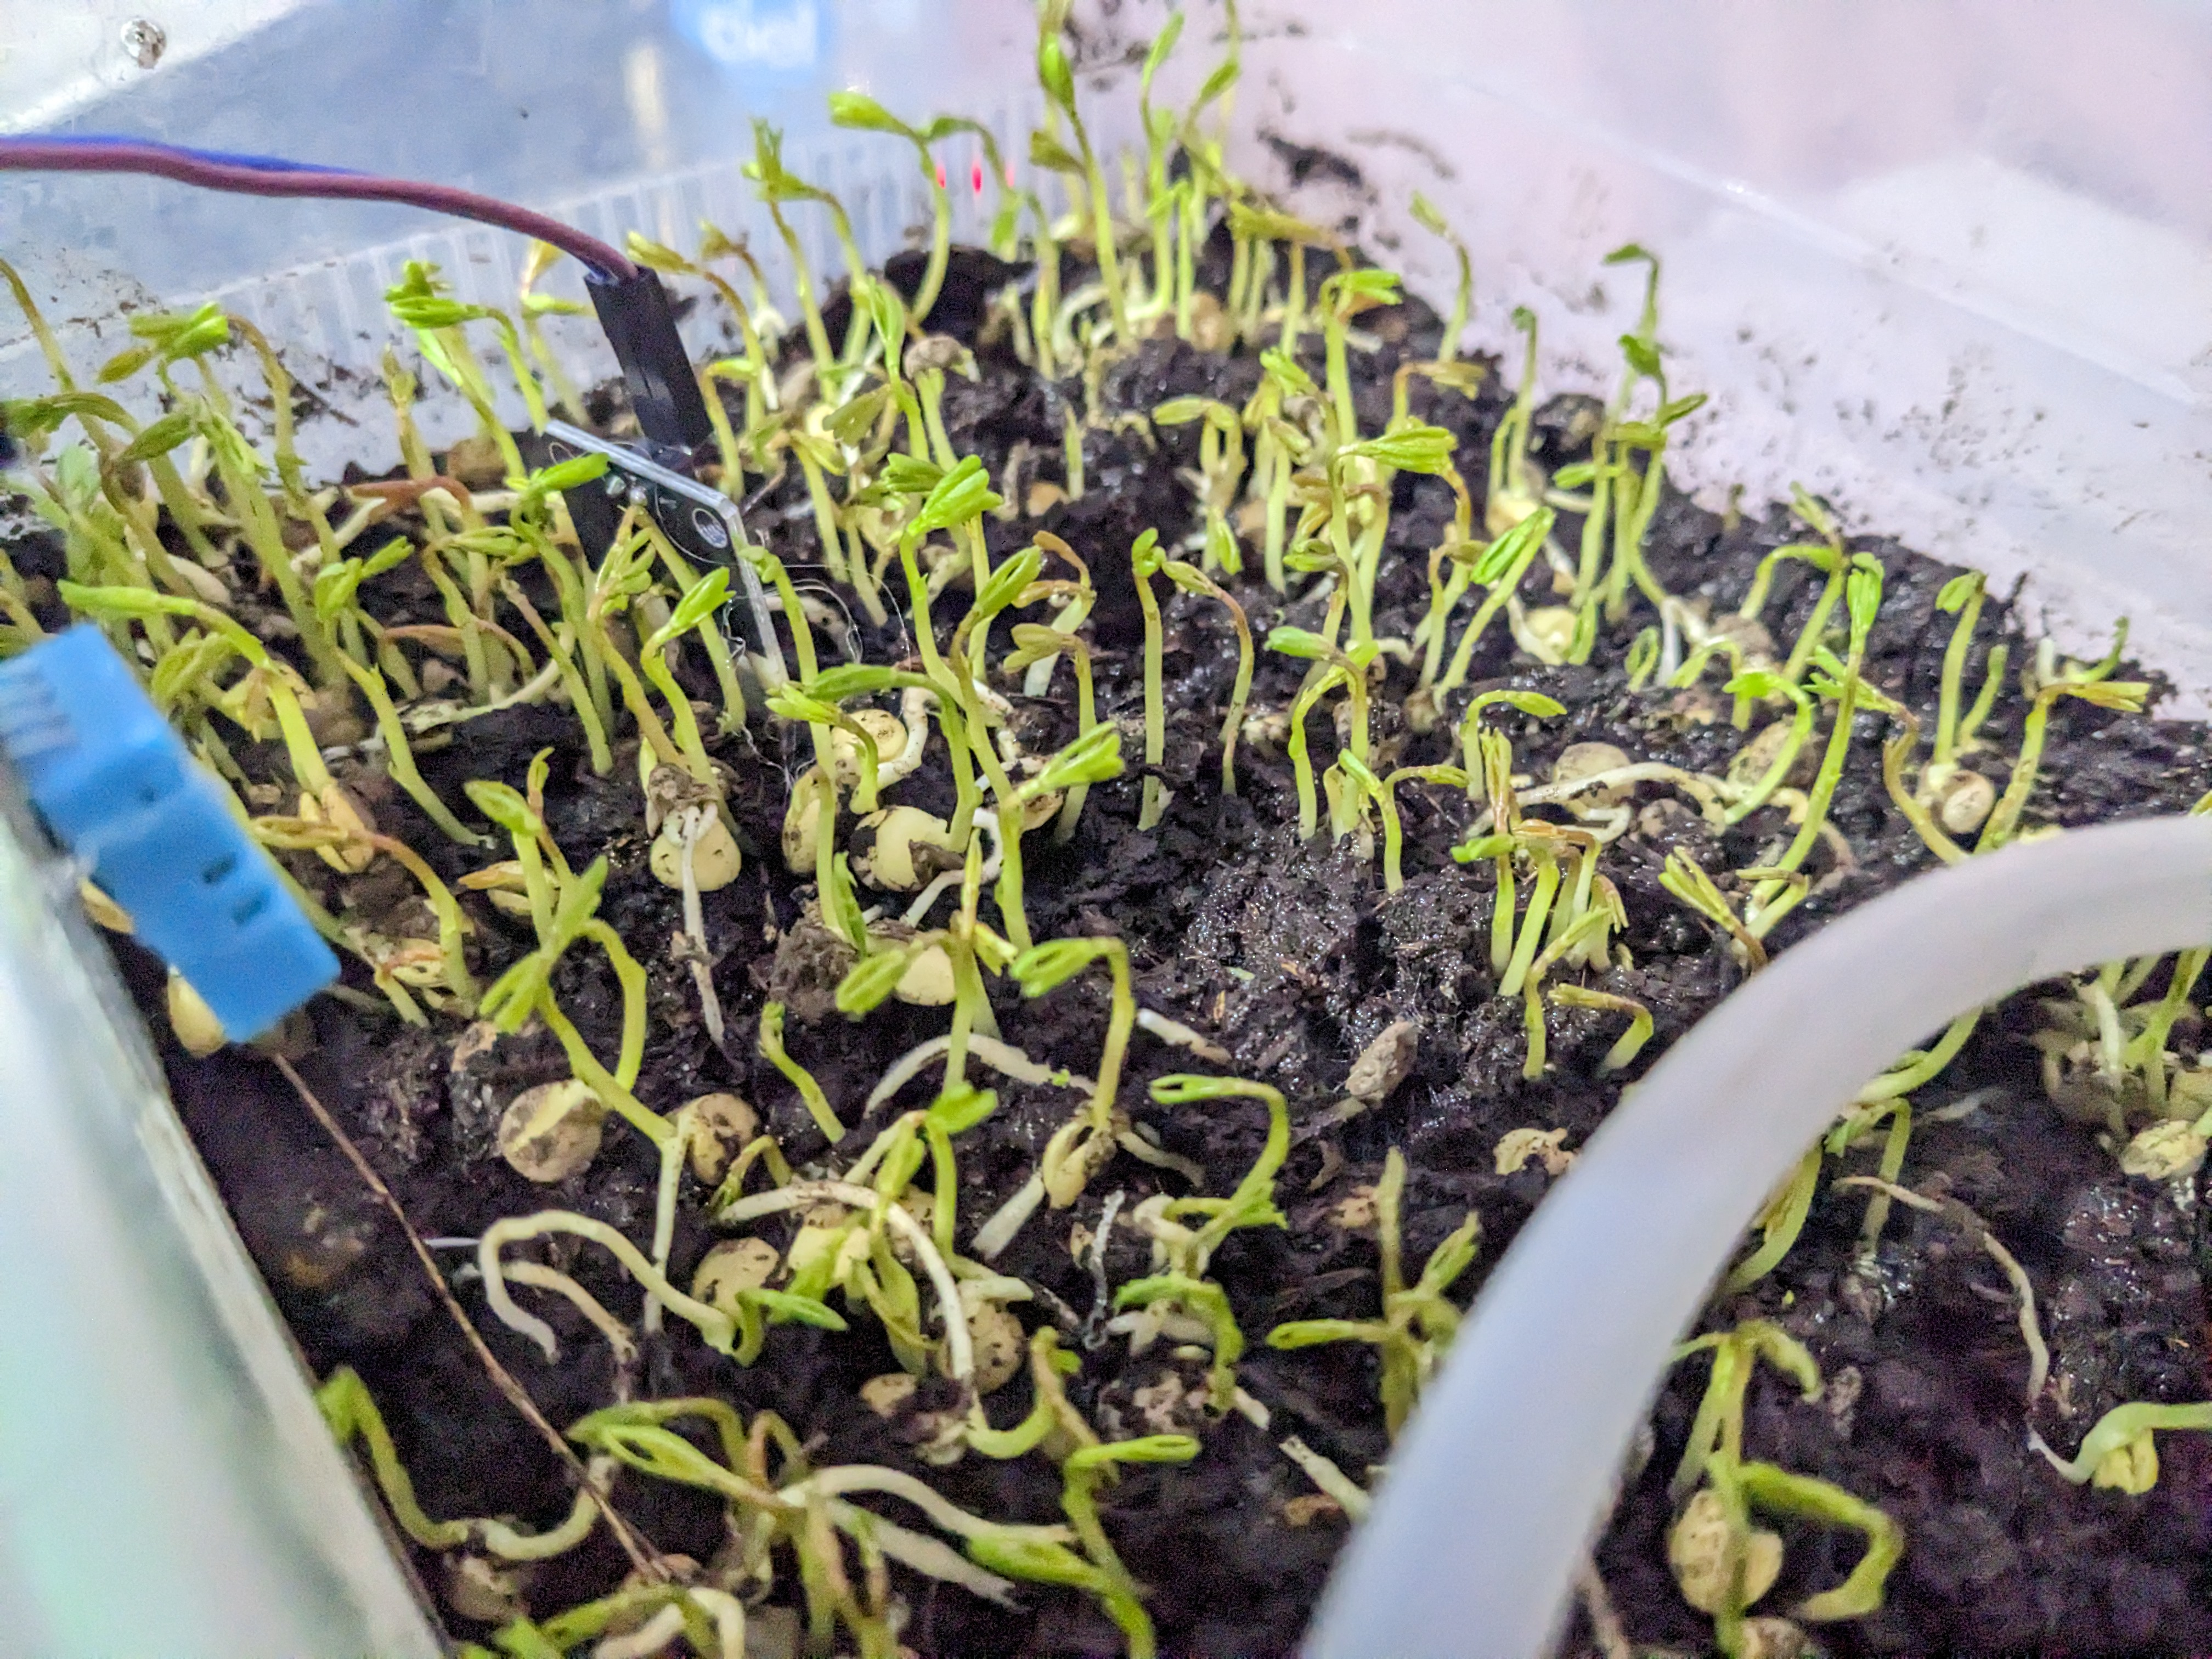
\includegraphics[width=\linewidth]{planta.jpg}
  \caption{Planta de lentejas que se cultivó con ayuda de Agrocare}
  \label{fig:example}
\end{figure}

También logramos proporcionar energía solar que ayudó a que el sistema sea autosustentable con una autonomía de aproximadamente 10 horas, suficiente para pasar la noche sin sol.

\section{Conclusiones}
En conclusión, los huertos urbanos y rurales se han vuelto una tendencia en la producción de alimentos debido a la conciencia ambiental y los efectos económicos de la pandemia por Covid-19. Sin embargo, su cuidado adecuado es un desafío, especialmente en el caso de los huertos rurales debido a la falta de atención constante y el alto costo de la tecnología de monitoreo. Es fundamental encontrar soluciones asequibles y eficaces para los productores y consumidores, lo que mejoraría la productividad y calidad de los cultivos, y reduciría el impacto negativo en el medio ambiente.\\

La tecnología actual, como los sensores de temperatura y humedad conectados a dispositivos de IoT, puede ser utilizada para el monitoreo y control remoto de los huertos. La implementación de tecnología en los huertos puede mejorar la productividad y calidad de los cultivos, además de tener un impacto positivo en el medio ambiente. Además, la recolección y análisis de datos en tiempo real permiten tomar decisiones y establecer estrategias para el cuidado de las plantas. El uso de Redes Neuronales Recurrentes permite ajustar los sesgos utilizando datos históricos y asegura la fidelidad de los datos, lo que resulta útil en proyectos como Agrocare.\\

El objetivo del proyecto es determinar si el cuidado de plantas automatizado con robótica es eficiente, escalable y sostenible a largo plazo. Con la ayuda de Agrocare, se espera medir los valores que afectan el crecimiento de una planta, incluyendo la humedad del suelo, humedad relativa, luz solar y temperatura. Posteriormente, estos datos serán analizados en un servidor remoto apoyándose de un microservicio de Red Neuronal Recurrente y una base de datos. El flujo de datos será automatizado y eficiente, lo que permitirá que el cuidado de las plantas sea escalable y sostenible a largo plazo. Este proyecto puede ser una solución asequible y eficaz para los productores y consumidores, lo que mejoraría la productividad y calidad de los cultivos y reduciría el impacto negativo en el medio ambiente.

\bibliographystyle{apacite}
\bibliography{bibliografia}

\section{Glosario}
\noindent\textbf{Inteligencia Artificial} (IA): Capacidad de máquinas y sistemas informáticos para realizar tareas mediante programación de algoritmos y técnicas de aprendizaje automático.

\noindent\textbf{Internet de las Cosas} (IoT): Interconexión de dispositivos físicos a través de Internet para interactuar con el mundo real y comunicarse entre sí.

\noindent\textbf{Microcontrolador}: Dispositivo programable que integra procesador, memoria y periféricos de entrada/salida, diseñado para controlar procesos específicos en tiempo real.

\noindent\textbf{Sensor}: Dispositivo que mide una magnitud física o química y convierte la información en una señal eléctrica o digital.

\noindent\textbf{Fotorresistencia} (LDR): Tipo de sensor que varía su resistencia eléctrica según la cantidad de luz que recibe, utilizado en sistemas de iluminación y control de exposición en fotografía.

\noindent\textbf{Capacitivo}: Tecnología de sensores que miden la capacidad de almacenamiento de carga eléctrica en un material dieléctrico, utilizados en pantallas táctiles y botones capacitivos.

\noindent\textbf{Red Neuronal Recurrente}: Modelo de inteligencia artificial de aprendizaje profundo utilizado en el procesamiento de secuencias de datos, como el reconocimiento del habla y el procesamiento del lenguaje natural.

\noindent\textbf{API}: Conjunto de reglas y protocolos que permiten la interacción y comunicación entre diferentes sistemas o aplicaciones de software, utilizadas para la integración de servicios y la automatización de tareas.

\noindent\textbf{\textit{Socket}}: Mecanismo de comunicación entre procesos en una red de computadoras, permitiendo el intercambio de información mediante protocolos de comunicación estándar.

\noindent\textbf{LCD}: Tipo de pantalla de visualización que utiliza cristales líquidos para mostrar imágenes y texto, comúnmente utilizadas en dispositivos electrónicos portátiles.

\noindent\textbf{Déficit Hídrico}: Condición adversa a la que se expone un cultivo cuando no hay agua suficiente.

\noindent\textbf{Estrés Hídrico}: Condición adversa a la que se expone un cultivo cuando el suelo está excesivamente húmedo.

\end{document}
